\chapter{Interfejs użytkownika}
\par W tym została wyjaśniona kwestia komunikacji z użytkownikiem końcowym za pomocą interfejsu. Znajdują się tutaj informację na temat wyświetlania danych na ekranie, zachowania programu w określonych sytuacjach oraz sterowania mikrokontrolerem przez użytkownika.
\section{Wygląd i obsługa}

\par Główny interfejs został podzielony na 3 karty menu, które są wybieralne przełącznikiem. Dodatkowo, w przypadku, gdy pojazd zatrzymał się, karta zmienia się automatycznie na alternatywną czwartą kartę, która pokazuje statystyki z przejazdu. Kolejną funkcjonalnością jest przytrzymanie przełącznika, które w zależności od aktualnej karty albo resetuje zapisane dane w pamięci, albo wyłącza podświetlenie ekranu.

\subsubsection{Pierwsza karta}

Zostało założone, że pierwsza karta będzie tą najczęściej używaną, więc znalazły się na niej najczęściej potrzebne parametry: prędkość, spalanie na 100km, temperatura, napięcie w układzie i położenie pedału gazu. Podgląd tej można zobaczyć na rysunku (rys.~\ref{fig:menu1}).

\begin{figure}[!htb]
\centering
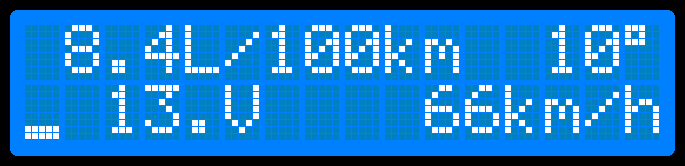
\includegraphics[width=0.7\linewidth]{Rysunki/menu1.png}
\caption{Podgląd pierwszej karty menu}
\label{fig:menu1}
\end{figure}

\subsubsection{Druga karta}
Na drugiej karcie znalazły się informacje na temat przejechanego dystansu oraz spalonego paliwa. Podgląd tej można zobaczyć na rysunku (rys.~\ref{fig:menu2}).

\begin{figure}[!htb]
\centering
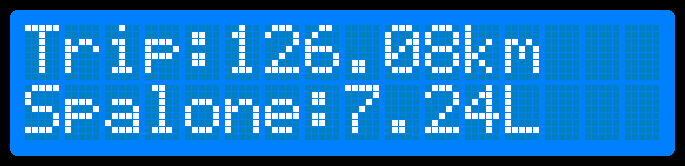
\includegraphics[width=0.7\linewidth]{Rysunki/menu2.png}
\caption{Podgląd drugiej karty menu}
\label{fig:menu2}
\end{figure}

\subsubsection{Trzecia karta}
Na trzeciej karcie znajdują się informacje na temat spalania: spalanie na 100 km, spalanie na godzinę oraz średnie spalanie na 100 km.Podgląd tej można zobaczyć na rysunku (rys.~\ref{fig:menu3}).

\begin{figure}[!htb]
\centering
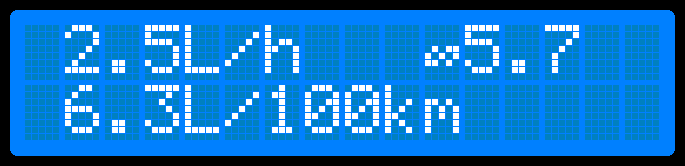
\includegraphics[width=0.7\linewidth]{Rysunki/menu3.png}
\caption{Podgląd trzeciej karty menu}
\label{fig:menu3}
\end{figure}


\subsubsection{Karta przy postoju}
Na tej karcie znalazły się informacje na temat średniego spalania, spalonego paliwa, aktualnego spalania na godzinę oraz przejechanego dystansu. Podgląd tej można zobaczyć na rysunku (rys.~\ref{fig:menu0}).

\begin{figure}[!htb]
\centering
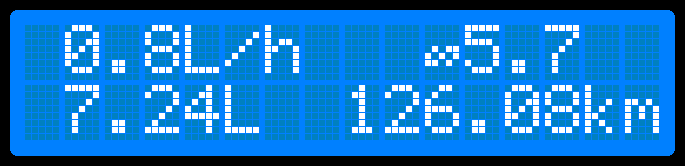
\includegraphics[width=0.7\linewidth]{Rysunki/menu0.png}
\caption{Podgląd postojowej karty menu}
\label{fig:menu0}
\end{figure}

Karta ta wyświetlana jest tylko wtedy, gdy prędkość pojazdu spadnie poniżej 2 km/h oraz przejechany dystans jest większy niż 200 m.

\section{Implementacja i formatowanie danych}
\subsubsection{Obsługa menu}

Obsłużenie kart menu polega na inkrementacji zmiennej \texttt{menu} podczas naciskania przycisku. W zależności wartości tej zmiennej wyświetlana jest inna karta menu.

\begin{lstlisting}[label=list:menu,caption=Implementacja obsługi menu,
basicstyle=\footnotesize\ttfamily]
int menu = 1;

void nacisnieciePrzycisku()
{
    if (menu > 3)
        menu = 1;
    else
        menu++;
}
---
void loop()
{
    ---
    switch (menu) 
    {
        case 1:
            menu1();
            break;
        case 2:
            menu2();
            break;
        case 3:
            menu2();
            break;
    }
    ---
}
\end{lstlisting}

\subsubsection{Włączanie postojowej karty}

\begin{lstlisting}[label=list:menu_card4,caption=Włączanie karty podczas postoju,
basicstyle=\footnotesize\ttfamily]
---
void loop()
{
    ---
    if (predkosc < 2.0 && trip > 0.2)
    {
        menu0();
    }
    ---
}
\end{lstlisting}
\subsubsection{Odświeżanie danych}
\par W przypadku, gdy odświeżanie wykonywałoby się bardzo szybko ekran LCD zacząłby migotać co utrudniałoby odczyt danych. Z tego powodu odświeżanie informacji na ekranie odbywa się co jedną sekundę. Zostało to zaimplementowane przy użyciu funkcji \texttt{millis()}, która zwraca liczbę milisekund od włączenia programu, podzielonej modulo 1000 (1 sekunda). W ten sposób, gdy wartość tego zapytania wynosi 0 przesyłane są nowe informacje do LCD.

\begin{lstlisting}[label=list:refresh_rate,caption=Implementacja odświeżania ekranu,
basicstyle=\footnotesize\ttfamily]
const czas_odswiezania_lcd = 1000;
---
void loop()
{
    ---
    if (millis() % czas_odswiezania_lcd == 0) 
    {
        // instrukcje dla wyświetlacza
    }
    ---
}

\end{lstlisting}

Jako, iż temperatura nie zmienia się tak szybko, a jej odczyt trwa chwilę czasu zostało postanowione, że będzie ona pobierana co 60 sekund oraz 2,5 sekundy po starcie programu.
\begin{lstlisting}[label=list:temp_refresh_rate,caption=Implementacja odświeżania temperatury,
basicstyle=\footnotesize\ttfamily]
const czas_odswiezania_temperatury = 60000;
float temp = 0.0;
---
void loop()
{
    ---
    if (millis() % czas_odswiezania_temperatury == 0 || millis() == 2500)
    {
        temp = temperatura();
    }
    ---
}

\end{lstlisting}

\subsubsection{Prędkość}
Do wyświetlania aktualnej prędkości w formacie \textit{XXXkm/h} została przygotowana funkcja \texttt{wyswietlaniePredkosci(int X, int Y)}, która przyjmuje parametry X i Y, które oznaczają współrzędne wyświetlenia prędkości na wyświetlaczu.
\begin{lstlisting}[label=list:show_speed,caption=Wyświetlanie prędkości,
basicstyle=\footnotesize\ttfamily]
void wyswietlaniePredkosci(int X, int Y)
{
    lcd.setCursor(X, Y);
    lcd.print(predkosc, 0);
    lcd.print("km/h");
    lcd.setCursor(X - 3, Y);
    lcd.print("   ");
    if (predkosc >= 0 && predkosc < 10)
    	lcd.setCursor(X - 1, Y);
    else if (predkosc >= 10 && predkosc < 100)
    	lcd.setCursor(X - 2, Y);
    else if (predkosc >= 100)
    	lcd.setCursor(X - 3, Y);
}
\end{lstlisting}
\subsubsection{Spalanie na 100km}
Do wyświetlania aktualnego spalania w formacie \textit{XX.XL/100km} została przygotowana funkcja \texttt{wyswietlanieSpalaniaNa100(int X, int Y)}, która przyjmuje parametry X i Y, które oznaczają współrzędne wyświetlenia spalania na wyświetlaczu.
\begin{lstlisting}[label=list:show_fuel_cons_100,caption=Wyświetlanie spalania na 100km,
basicstyle=\footnotesize\ttfamily]
void wyswietlanieSpalaniaNa100(int X, int Y)
{
    lcd.setCursor(X + 4, Y);
    lcd.print("L/100km");
    lcd.setCursor(X + 1, Y);
    if (predkosc < 5)
    	lcd.print("0.0");
    else
    {
    	if (spalanieSto < 10)
    		lcd.print(spalanieSto, 1);
    	else if (spalanieSto >= 10)
    	{
    		lcd.setCursor(X, Y);
    		lcd.print(spalanieSto, 1);
    	}
    }
}
\end{lstlisting}

\subsubsection{Spalanie na godzinę}
Do wyświetlania aktualnego spalania w formacie \textit{X.XL/h} została przygotowana funkcja \texttt{wyswietlanieSpalaniaNaGodzine(int X, int Y)}, która przyjmuje parametry X i Y, które oznaczają współrzędne wyświetlenia spalania na wyświetlaczu.
\begin{lstlisting}[label=list:show_fuel_cons_hour,caption=Wyświetlanie spalania na godzinę,
basicstyle=\footnotesize\ttfamily]
void wyswietlanieSpalaniaNaGodzine(int X, int Y)
{
    lcd.setCursor (X + 3, Y);
	lcd.print("L/h");
	lcd.setCursor (X, Y);
	lcd.print(spalanieH, 1);
}
\end{lstlisting}

\subsubsection{Temperatura}
Do wyświetlania temperatury w formacie \textit{XX°} została przygotowana funkcja \texttt{wyswietlanieTemperatury(int X, int Y)}, która przyjmuje parametry X i Y, które oznaczają współrzędne wyświetlenia temperatury na wyświetlaczu.
\begin{lstlisting}[label=list:show_tempr,caption=Wyświetlanie temperatury,
basicstyle=\footnotesize\ttfamily]
void wyswietlanieTemperatury(int X, int Y)
{
    lcd.setCursor(X + 3, Y);
    lcd.print((char)223);
    lcd.setCursor(X, Y);
    lcd.print("   ");
    if (temp < 10 && temp >= 0)
    	lcd.setCursor(X + 2, Y);
    else if (temp >= 10 || (temp < 0 && temp >= -10) )
    	lcd.setCursor(X + 1, Y);
    else if (temp <= 10)
    	lcd.setCursor(X, Y);
    lcd.print(temp, 0);
}
\end{lstlisting}

\subsubsection{Napięcie}
Do wyświetlania aktualnego napięcia w formacie \textit{XX.XV} została przygotowana funkcja \texttt{wyswietlanieNapiecia(int X, int Y)}, która przyjmuje parametry X i Y, które oznaczają współrzędne wyświetlenia napięcia na wyświetlaczu.
\begin{lstlisting}[label=list:show_voltage,caption=Wyświetlanie napięcia,
basicstyle=\footnotesize\ttfamily]
void wyswietlanieNapiecia(int X, int Y)
{
    lcd.setCursor(X, Y);
    lcd.print(woltomierz(),1);
    lcd.setCursor(X + 4, Y);
    lcd.print("V");
}
\end{lstlisting}

\subsubsection{Przejechany dystans}
Do wyświetlania przejechanego dystansu w formacie \textit{XXXkm} została przygotowana funkcja \texttt{wyswietlanieDystansu(int X, int Y)}, która przyjmuje parametry X i Y, które oznaczają współrzędne wyświetlenia dystansu na wyświetlaczu.
\begin{lstlisting}[label=list:show_millage,caption=Wyświetlanie dystansu,
basicstyle=\footnotesize\ttfamily]
void wyswietlanieDystansu(int X, int Y)
{
    lcd.setCursor(X, Y);
    lcd.print(trip);
    lcd.print("km");
}
\end{lstlisting}

\subsubsection{Spalone paliwo}
Do wyświetlania spalonego paliwa w formacie \textit{XX.XL} została przygotowana funkcja \texttt{wyswietlanieSpalonegoPaliwa(int X, int Y)}, która przyjmuje parametry X i Y, które oznaczają współrzędne wyświetlenia spalonego paliwa na wyświetlaczu.
\begin{lstlisting}[label=list:show_fuel_burned,caption=Wyświetlanie spalonego paliwa,
basicstyle=\footnotesize\ttfamily]
void wyswietlanieSpalonegoPaliwa(int X, int Y)
{
    lcd.setCursor(X, Y);
    lcd.print(spalone, 2);
    if(spalone < 10)
    	lcd.setCursor (X + 4, Y);
    else
    	lcd.setCursor (X + 4, Y);
    lcd.print("L");
}
\end{lstlisting}

\subsubsection{Średnie spalanie na 100 km}
Do wyświetlania średniego spalonego paliwa na 100 km w formacie \textit{•XX.X} została przygotowana funkcja \texttt{wyswietlanieSredniegoSpalania(int X, int Y)}, która przyjmuje parametry X i Y, które oznaczają współrzędne wyświetlenia średniego spalonego paliwa na wyświetlaczu.
\begin{lstlisting}[label=list:show_fuel_avarge,caption=Wyświetlanie średniego spalonego paliwa na 100km,
basicstyle=\footnotesize\ttfamily]
void wyswietlanieSredniegoSpalania(int X, int Y)
{
    lcd.setCursor (X, Y);
    lcd.print((char)243);
    lcd.setCursor (X + 1, 1);
    if (trip == 0.0)
    	lcd.print("0.0");
    else
    	lcd.print((100/trip)*spalone, 1);
}
\end{lstlisting}

\subsubsection{Położenie pedału gazu}
Kontroler sterujący wyświetlaczem umożliwia manualne stworzenie znaków. Dzięki tej opcji zostały stworzone specjalne znaki, które graficznie pokazują nacisk pedału. Działają one na zasadzie paska postępu, który ładuje się z dołu do góry w zależności od wciśnięcia pedału gazu.

\begin{lstlisting}[label=list:custom_char,caption=Tworzenie znaków specjalnych dla odczytu pedału gazu,
basicstyle=\footnotesize\ttfamily]
byte a1[8] = {B00000,B00000,B00000,B00000,B00000,B00000,B00000,B11111};
byte a2[8] = {B00000,B00000,B00000,B00000,B00000,B00000,B11111,B11111};
byte a3[8] = {B00000,B00000,B00000,B00000,B00000,B11111,B11111,B11111};
byte a4[8] = {B00000,B00000,B00000,B00000,B11111,B11111,B11111,B11111};
byte a5[8] = {B00000,B00000,B00000,B11111,B11111,B11111,B11111,B11111};
byte a6[8] = {B00000,B00000,B11111,B11111,B11111,B11111,B11111,B11111};
byte a7[8] = {B00000,B11111,B11111,B11111,B11111,B11111,B11111,B11111};
byte a8[8] = {B11111,B11111,B11111,B11111,B11111,B11111,B11111,B11111};
---
void setup()
{
    ---
    lcd.createChar(0, a1);
	lcd.createChar(1, a2);
	lcd.createChar(2, a3);
	lcd.createChar(3, a4);
	lcd.createChar(4, a5);
	lcd.createChar(5, a6);
	lcd.createChar(6, a7);
	lcd.createChar(7, a8);
    ---
}
\end{lstlisting}

Do wyświetlania aktualnego położenia pedału gazu została przygotowana funkcja \texttt{wyswietlaniePolozeniaPedaluGazu(int X, int Y)}, która przyjmuje parametry X i Y, które oznaczają współrzędne wyświetlenia odczytu na wyświetlaczu.
\begin{lstlisting}[label=list:show_fuel_avarge,caption=Wyświetlanie średniego spalonego paliwa na 100km,
basicstyle=\footnotesize\ttfamily]
float nacisk = 0.0;
void wyswietlaniePolozeniaPedaluGazu(int X, int Y)
{
    nacisk = aktualnyNacisk();
    lcd.setCursor (X, Y);
    if (nacisk <= 3)
    	lcd.print(" ");
    else if (nacisk > 3 && nacisk <= 12.5)
    	lcd.write(byte(0));
    else if (nacisk > 12.5 && nacisk <= 25)
    	lcd.write(byte(1));
    else if (nacisk > 25 && nacisk <= 37.5)
    	lcd.write(byte(2));
    else if (nacisk > 37.5 && nacisk <= 50)
    	lcd.write(byte(3));
    else if (nacisk > 50 && nacisk <= 62.5)
    	lcd.write(byte(4));
    else if (nacisk > 62.5 && nacisk <= 75)
    	lcd.write(byte(5));
    else if (nacisk > 75 && nacisk <= 87.5)
    	lcd.write(byte(6));
    else if (nacisk > 87.5)
    	lcd.write(byte(7));
    }
}
\end{lstlisting}

\subsubsection{Resetowanie zapisanych danych}
W celu umożliwienia użytkownikowi zerowania zapisanych danych została stworzona funkcja \texttt{resetuj()}. Można ją wywołać przytrzymując przycisk jednocześnie będąc na 2 karcie menu.

\begin{lstlisting}[label=list:menu_card4,caption=Resetowanie zapisanych danych,
basicstyle=\footnotesize\ttfamily]
---
void resetuj()
{
    EEPROMWritelong(0, 0);
    EEPROMWritelong(4, 0);
    dystans = 0;
    trip = 0;
}
void przytrzymaniePrzycisku()
{
    switch (menu)
    {
    ---
    case 2:
        resetuj();
        break;
    ---
    }
}
---
\end{lstlisting}

\subsubsection{Sterowanie podświetleniem}
Moduł umożliwia również sterowanie podświetleniem poprzez zmianę stanu portu. Zostały stworzone dwa tryby podświetlenia: domyślny (pełna jasność) oraz wyłączony (nocny). Można je przełączać przytrzymaniem przycisku, gdy aktualną kartą menu jest karta pierwsza.

\begin{lstlisting}[label=list:hold_button_brightness,caption=Resetowanie zapisanych danych,
basicstyle=\footnotesize\ttfamily]
bool jasnosc = true;
const jasnosc_pin = 9;
---
void setup()
{
    ---
    digitalWrite(jasnosc_pin, jasnosc);
    ---
}
void przelaczPodswietlenie()
{
    jasnosc = !jasnosc;
    digitalWrite(jasnoscPin, jasnosc);
}
void przytrzymaniePrzycisku()
{
    switch (menu)
    {
    ---
    case 1:
        przelaczPodswietlenie();
        break;
    ---
    }
}
---
\end{lstlisting}